\documentclass[twoside,letterpaper,11pt]{article}

\usepackage{mystyle}
\newcommand{\sgrad}{\nabla_{\sigma}}
% TODO make the background of theorems darker (or at least make sure that the
% printer does).
\usepackage{wrapfig}
\newcommand{\KAM}{ Let $\rho, \gamma > 0$ be given, and let
  $h(\bp{q}, \bp{p}) = h_0(\bp{p}) + h_1(\bp{q}, \bp{p})$ be a Hamiltonian, with
  $h_0, h_1 \in \mathcal{A}_{\rho}$ and $\norm{h}_{\rho} \leq 1$.
  Suppose the Taylor polynomial of $h_0$ is
  \begin{equation*}
    h_0(\bp{p}) = a + \omega\bp{p} + \frac{1}{2} \bp{p} \cdot C \bp{p} +
    o(|\bp{p}|^2),
  \end{equation*}
  with $\omega \in \Omega_{\gamma}$ and $C$ is symmetric and invertible.
  Then for any $\rho_* \leq \rho$, there exists $\epsilon > 0$, which depends on
  $C$ and $\gamma$, but not on the remainder term in $o(|\bp{p}|^2)$, such that
  if $\norm{h_1}_{\rho} \leq \epsilon$, there exists a symplectic mapping $\Phi
  : A_{\rho_*} \to A_{\rho}$ such that if we set $(\bp{q}, \bp{p}) = \Phi(\bp{Q},
  \bp{P})$ and $H = h \circ \Phi$, we have
  \begin{equation*}
    H(\bp{Q}, \bp{P}) = A + \omega \bp{P} + R(\bp{Q}, \bp{P}),
  \end{equation*}
  with $R(\bp{Q}, \bp{P}) \in O(|\bp{P}|^2)$.
}

\newcommand{\dionumber}{
  A number $\theta$ is \emph{Diophantine of exponent d} if there exists a
    constant $\gamma > 0$ such that for all coprime integers $p$ and $q$ we have
    \begin{equation*}
      \left| \theta - \frac{p}{q} \right| > \frac{\gamma}{|q|^d}.
    \end{equation*}
}

\newcommand{\diovector}{
  Let $\omega = (\omega_1, \ldots, \omega_n)$.
    We say $\omega$ is Diophantine if there exists $\gamma > 0$ such that for
    all vectors with integer coefficients $(k_1, \ldots, k_n)$, we have
    \begin{equation*}
      |k_1 \omega_1 + \cdots + k_n \omega_n| \geq \frac{\gamma}{(k_1^2 + \cdots
        + k_n^2)^{\frac{n}{2}}}.
    \end{equation*}
    Let $\Omega_{\gamma}^n$ be the subset of such $\omega \in \R^n$.
}

\newcommand{\domains}{
  \begin{align*}
    B_{\rho} &= \{\bp{p} \in \C : |\bp{p}| \leq \rho\},\\
    C_{\rho} &= \{\bp{q} \in \C^n / \Z^n : | \Imag(\bp{q}) | \leq \rho\},\\
    A_{\rho} &= C_{\rho} \times B_{\rho} = \{(\bp{q}, \bp{p}) \in \C^n / \Z^n
               \times \C^n : |\bp{p}| \leq \rho, \, |\Imag(\bp{q})| \leq \rho\}.
  \end{align*}
}



\numberwithin{equation}{section}

\newcommand{\T}{\mathbb{T}}

\usepackage{fancyhdr}
\setlength{\headheight}{14.0pt}
\setlength{\headsep}{0.2in}
\renewcommand{\headrulewidth}{0pt}
\cfoot{}
\pagestyle{fancy}

\renewcommand{\sectionmark}[1]{ \markright{Section \thesection. #1}{} }

\fancyhf{}
\fancyhead[LE]{\textsc{\thepage \qquad \nouppercase{\rightmark}} }
\fancyhead[RO]{\textsc{Travis Westura \qquad \thepage}}

\fancypagestyle{plain}{ %
  \fancyhf{}
  \renewcommand{\headrulewidth}{0pt}
  \renewcommand{\footrulewidth}{0pt}
}

\title{Kolmogorov's Theorem}
\author{Travis Westura}
\date{\today}

\begin{document}

\maketitle

% I know that I'm not supposed to use a citation in an abstract, but Hubbard
% did so in his paper, so I guess it is fair game.
\begin{abstract}
  This paper discusses a proof of Kolmogorov's Theorem on the conservation of
  invariant tori.
  We follow the approach given by Hubbard and Ilyashenko in \cite{hi02}.
  Their proof is influenced by the one given by Bennettin, Galgani, Giorgilli,
  and Strelcyn in \cite{bggs84}, which itself resembles Kolmogorov's original
  argument.
\end{abstract}

\section{Introduction}
\label{sec:introduction}

Andrey Kolmogorov announced an important theorem about the conservation of
invariant tori in the International Congress of Mathematicians in $1954$
\cite{kol54}.
However, he never wrote down a proof of this theorem.
Vladimir Arnold give a proof in $1963$, and J{\"u}rgen Moser proved a related
result in $1962$.
The resulting theory is therefore called KAM Theory, named after the three of
them.

Arnold recalls in \cite{a97} how Kolmogorov had been considering the problem
since he was a child.
He was influenced by reading \emph{The Flammarion Book of Astronomy}, where
\cite{f64} is a more recent edition than the one Kolmogorov would have read.
After Stalin died Kolmogorov entered a period of great mathematical
productivity.
This theorem was born out of this period.

While Kolmogorov never wrote down a proof, many others did, or at least
attempted to.
As already noted, Arnold wrote a proof \cite{a63} in $1963$ and Moser proved a
related result \cite{mos62} in $1962$.
But the proof is quite difficult, as Arnold's original argument was over $60$
pages and quite difficult to understand.
The argument with which we concern ourselves is given by Hubbard and Ilyshenko
in \cite{hi02}.
This proof, while still containing many messy, technical details, is much
shorter.
We will discuss the motivation behind the main ideas and key concepts of this
proof.

Before moving on, let's take a look at our main goal:
\begin{thm}[Kolmogorov's Theorem]
  \label{thm:KAM}
  \KAM{} In particular the torus $\bp{P} = 0$ is invariant under the flow
  $\sgrad H$, and on this torus the flow $\phi_H$ is linear with direction
  $\omega$.
\end{thm}
We will return to this statement after building up some intuition for it.
For now, let's just note that the proof involves solving \cref{eq:sdiffeo} for
the symplectic diffeomorphism $\Phi$.

We will begin by examining a toy example of the solar system, to which we will
apply the theorem.
This example will help us in understanding the statement of the theorem and the
tools that we will need in the proof.
We will discuss the basics of Hamiltonian mechanics and the notion of irrational
vectors while examining this example.
Then we will begin examining the technique of the proof and examine the role
played by analytic functions.
Finally we will put all of this together and explain the main ideas of the
proof, while leaving out some of the more messy, technical details.

\section{A Motivating Example}
\label{sec:motivating-example}

To start understanding the theorem, let's consider an example to which we would
like to apply it.
While staring up at the night sky, one might be driven to wonder, ``Why do the
planets orbit around the sun and not just crash into it or fly off by themselves
in their own directions?''
Kolmogorov's Theorem gives us a method to attempt to answer this question.

Let's start by discussing a simplified model of our solar system.
In this model we will assume that planets have zero mass.
This assumption is reasonable, as the masses of the planets are extremely small
compared to that of the sun.
Indeed, the sun is so massive compared to the planets that Jupiter and the sun
orbit around a point that is located inside of the surface of the sun.
Thus we may, at least for the moment, consider these masses to be negligible.

A system with $n$ bodies, each with a mass $m_i$ and a position $\bp{x}_i$,
satisfies Netwon's second law: $\bp{F} = m \bp{a}$.
For each $i$, we have
\begin{equation*}
  m_i \bdd{x} = \sum_{j \neq i} \mathrm{G} \nobreak\hspace{.125em plus
    .14286em} m_i m_j \frac{\bp{x}_j - \bp{x}_i}{|\bp{x}_j - \bp{x}_i|^3}.
\end{equation*}
Here, $\mathrm{G} \approx 6.62 \cdot 10^{-11} m^3 / (kg\, s^2)$ is the universal
gravitational constant.
On the left hand side we have each planet's mass and its acceleration.
On the right hand side we have the force that acts on this mass.
Note that the force is inversely proportional to the square of the distances
between the forces.
The top of the fraction contains the vector $\bp{x}_j - \bp{x}_i$ that has
length $|\bp{x}_j - \bp{x}_i|$.
To cancel out this length, we divide by $|\bp{x}_j - \bp{x}_i|^3$.
This gives us the desired inverse proportionality to the square of the distance.

In our model of the solar system we take the sun to be given by the index $0$
and the planets given by indices from $1$ to $8$ or $9$, depending on the
reader's opinions of Pluto.
Now we will examine what happens as the masses of the planets, the $m_j$ for $j
= 1, \ldots, n$, tend to zero.

Rewriting the previous equations, we have
\begin{align*}
  \bdd{x}_0 &= \mathrm{G} \sum_{j = 1}^n m_j \frac{\bp{x}_j -
              \bp{x}_0}{|\bp{x}_j = \bp{x}_i|^3},\\
  \bdd{x}_i &= \mathrm{G} m_0 \frac{\bp{x}_0 - \bp{x}_i}{|\bp{x}_0 -
              \bp{x}_i|^3} + \mathrm{G} \nobreak\hspace{.125em plus
              .14286em}
              \sum_{\mathclap{\substack{j=1,\ldots,n\\j\neq i}}}
              m_j \frac{\bp{x}_j - \bp{x}_i}{|\bp{x}_j - \bp{x}_i|^3}.
\end{align*}
Now we keep the mass of the sun $m_0$ constant but let the masses of the planets
go to zero.
These equations then become
\begin{align*}
  \bdd{x}_0 &= 0,\\
  \bdd{x}_j &= \mathrm{G} \nobreak\hspace{.125em plus .14286em} \frac{\bp{x}_0 -
              \bp{x}_i}{|\bp{x}_0 - \bp{x}_i|^3}.
\end{align*}
We can even simplify these equations a bit further.
Since $\bdd{x}_0 = 0$, the body with mass $m_0$ travels in a straight line with
constant speed.
Thus we can work in a heliocentric system of coordinates with the sun at the
center of our solar system with position $\bp{x}_0 = 0$.
We then have
\begin{align*}
  \bdd{x}_0 &= 0,\\
  \bdd{x}_j &= - \mathrm{G} \nobreak\hspace{.125em plus .14286em}
              m_0 \frac{\bp{x}_i}{|\bp{x}_i|^3}.
\end{align*}
In particular we can note that this system is stable.
Over time, it will never diverge far from its present state.

This model will serve as an example to which we apply the properties of
Hamiltonian Mechanics that are discussed in \cref{sec:hamilt-mech}.
Kolmogorov's theorem will then be applied in the context of this example in
\cref{sec:kam-solar-system}.

\section{Hamiltonian Mechanics}
\label{sec:hamilt-mech}

We will need to consider Hamiltonian mechanics in our study of the KAM Theorem.
Hamiltonian mechanics is a reformulation of Newtonian mechanics, named for
William Rowan Hamilton.
The theories produce the same results, but often one of them is a more
convenient formulation for some problems than is the other.

A Hamiltonian mechanical system is given by an even-dimensional manifold, the
phase space, a symplectic structure on this manifold, and a function $H$.
This function is called a Hamiltonian function.

Let $(X, \sigma)$ be a symplectic manifold.
That is, let $X$ be a differentiable manifold and $\sigma$ be a nowhere
vanishing $2$-form such that $\dif \sigma = 0$.
A function $H$ on $X$ has a \emph{symplectic gradient}, denoted $\sgrad H$.
This gradient is defined as the unique vector field $\sgrad H$ such that for any
vector field $\xi$, we have
\begin{equation}
  \label{eq:symplectic-grad}
  \sigma(\xi, \sgrad H) = \dif H(\xi).
\end{equation}
We will be considering a \emph{Hamiltonian differential equation} that makes use
of this symplectic gradient:
\begin{equation}
  \label{eq:hamiltonian-diff-eq}
  \bd{x} = (\sgrad H) (\bp{x}).
\end{equation}

Before moving on, let's compare the symplectic gradient and the gradient $\nabla
f$ of a function $f : \R^n \to \R$.
This gradient is not an element of $\R$, but rather is the vector
\begin{equation*}
  \nabla f =
  \begin{bmatrix}
    \pd{f}{x_1}\\
    \vdots\\
    \pd{f}{x_n}
  \end{bmatrix}.
\end{equation*}
In the symplectic gradient, we used the symplectic form $\sigma$ to give a
geometric structure to our underlying space.
Similarly, we can define the gradient by using the scalar product $\langle
\cdot, \cdot \rangle$ to provide a geometric structure.
In comparison to \cref{eq:symplectic-grad}, the gradient $\nabla f$ is the
unique vector field such that
\begin{equation*}
  \dif f(\xi) = \langle \xi, \nabla f \rangle.
\end{equation*}
Further, just as we considered a Hamiltonian differential equation in
\cref{eq:hamiltonian-diff-eq}, we can consider a gradient differential equation:
\begin{equation*}
  \bd{x} = \nabla f(\bp{x}).
\end{equation*}
The gradient and Hamiltonian differential equations are fundamentally different.
In the gradient equation, our function $f$ increases along solutions.
Thus these solutions may never return to their starting points.
The gradient differential equation prohibits any type of recurrence from
occurring.
In contrast, the Hamiltonian differential equation not just allows but
practically imposes recurrent behavior.
This difference means we can observe much more interesting recurrent behavior
when using Hamilton's equation than we could with the gradient equation.

As an example of a Hamiltonian system, let's consider our toy model of the solar
system from \cref{sec:motivating-example}.
We take our manifold $X$ to be $\R^{2n}$ with coordinates $(q_1, \ldots, q_n,
p_1, \ldots, p_n)$.
Our symplectic form will be given by
\begin{equation*}
  \sigma = \sum_{i} \dif p_i \wedge \dif q_i.
\end{equation*}
The Hamiltonian differential equation then becomes the \emph{Hamiltonian
  equations of motion}:
% TODO could talk about the Math $4200$ two dimensional case of Hamiltonian vs
% gradient systems
\begin{equation}
  \label{eq:hamiltonian-motion-eq}
  \begin{aligned}
    \dot{q}_i &= \pd{H}{p_i},\\
    \dot{p}_i &= - \pd{H}{q_i}.
  \end{aligned}
\end{equation}

Now we consider the case of a single body of zero mass.
It is sufficient to consider the single body system, since the planets' having
zero mass means that they do not affect each other in our toy system.
For $\bp{x} \in \R^2$, the equation
\begin{equation*}
  \bdd{x} = - \frac{\bp{x}}{|\bp{x}|^3}
\end{equation*}
is Hamilton's equation for the manifold $X = \R^2 \times \R^2$ with points
$(\bp{q}, \bp{p})$, standard symplectic form
\begin{equation*}
  \sigma = \dif p_1 \wedge \dif q_1 + \dif p_2 \wedge \dif q_2,
\end{equation*}
and Hamiltonian
\begin{equation*}
  H(\bp{q}, \bp{p}) = \frac{1}{2} (p_1^2 + p_2^2) - \frac{1}{\sqrt{q_1^2 +
      q_2^2}}.
\end{equation*}
We write $\bp{p} = \pt{p_1\\ p_2}$ and $\bp{q} = \pt{q_1\\q_2}$.
Now we have
\begin{align*}
  (\dif p_1 \wedge \dif q_1 &+ \dif p_2 \wedge \dif q_2)
                              \left(\left(\pt{\xi_1\\\xi_2}, \pt{\eta_1\\\eta_2}
  \right), \left( \pt{p1\\p2}, - \frac{1}{(q_1^2 + q_2^2)^{\frac{3}{2}}}
  \pt{q1\\q2} \right)\right)\\
                            &= \eta_1 p_1 + \frac{\xi_1 q_1}{(q_1^2 +
                              q_2^2)^{\frac{3}{2}}} + \eta_2 p_2 + \frac{\xi_2
                              q_2}{(q_1^2 + q_2^2)^{\frac{3}{2}}}\\
                            &= \left[ \Dif H \left( \pt{q1\\q1}, \pt{p1\\p2}
  \right) \right] \left( \pt{\xi_1\\\xi_2}, \pt{\eta_1\\\eta_2} \right).
\end{align*}
Following from this computation, we see that
\begin{equation*}
  \sgrad H = \left(\bp{p}, - \frac{1}{(q_1^2 + q_2^2)^{\frac{3}{2}}}\bp{q}
  \right).
\end{equation*}
The Hamiltonian differential equation $\bp{x} = \sgrad H(\bp{x})$ is then given
by
\begin{align*}
  q_1' &= p_1\\
  p_1' &= - \frac{q_1}{(q_1^2 + q_2^2)^{\frac{3}{2}}},\\
  q_2' &= p_2\\
  p_2' &= -\frac{q_2}{(q_1^2 + q_2^2)^{\frac{3}{2}}}.
\end{align*}
From here, we can recover the desired $\bdd{x} = - \frac{\bp{x}}{|\bp{x}|^3}$.

Now let's again consider the Hamiltonian differential equation given by
\cref{eq:hamiltonian-diff-eq}.
The vector field $\sgrad f$ has a flow that we denote by $\phi_f^t$.
This flow has two properties:
\begin{itemize}
\item $\phi_f^t$ preserves $f$: $f \circ \phi_f^t = f$,
\item $\phi_f^t$ preserves $\sigma$: $(\phi_f^t)^* \sigma = \sigma$.
\end{itemize}
Flows will be central to our proof of Kolmogorov's Theorem.
We will be constructing a symplectic diffeomorphism and will need the flows of
Hamiltonian functions to do so.

Further, in our proof we will be constructing Taylor polynomials of functions of
the form
\begin{equation*}
  t \mapsto g \circ \phi_f^t.
\end{equation*}
To perform this construction, we will use the Poisson bracket.
\begin{defn}[Poisson Bracket]
  Let $f$ and $g$ be two functions on $X$.
  The Poisson bracket, denoted $\{f, g\}$, is defined by
  \begin{equation*}
    \{f, g\} = \sigma(\sgrad f, \sgrad g) = \dif f(\sgrad g) = - \dif g(\sgrad
 f).
  \end{equation*}
\end{defn}
We say that two functions $f$ and $g$ commute if their Poisson bracket is zero:
\begin{equation*}
  \{f, g\} = 0.
\end{equation*}
The functions' commuting implies that their flows also commute:
\begin{equation*}
  \phi_f(s) \circ \phi_g(t) = \phi_g(t) \circ \phi_f(s).
\end{equation*}
The Poisson bracket allows to write Taylor polynomials in the form
\begin{equation*}
  f \circ \phi_g^t = f + t\{f, g\} + \frac{t^2}{2} \{\{f, g\}, g\} +
  \frac{t^3}{3!} \{ \{ \{f, g\}, g\}, g\} + \cdots.
\end{equation*}

The Poisson bracket is related to the Lie bracket:
the Lie bracket is the symplectic gradient of the Poisson bracket.
\begin{prop}[Relation of Poisson and Lie Brackets]
  For any two functions $f$ and $g$ on a symplectic manifold $(X, \sigma)$, we
  have
  \begin{equation*}
    \sgrad \{f, g\} = [\sgrad f, \sgrad g].
  \end{equation*} 
\end{prop}
\begin{proof}
  This proof will use the Jacobi identity for the Poisson bracket:
  \begin{equation*}
    \{\{f, g\}, h\} + \{\{g, h\}, f\} + \{\{h, f\}, g\} = 0.
  \end{equation*}
  This identity can itself be proved by a messy computation.

  Given a function $h$, we can compute
  \begin{align*}
    \dif h([\sgrad f, \sgrad g]) &= \dif (\dif h (\sgrad h)) (\sgrad f) - \dif
                                   (\dif h (\sgrad f)) (\sgrad g)\\
                                 &= \dif \{h, g\} (\sgrad f) - \dif \{h, f\}
                       (\sgrad g)\\
                                 &= \{ \{h, g\}, f\} - \{ \{ h, f\}, g\}\\
                                 &= \{\{h, g\}, f\} + \{\{f, h\}, g\}\\
                                 &= \{\{f, g\}, h\}\\
                                 &= \dif h (\sgrad \{f, g\}).
  \end{align*}
\end{proof}

As an example of a Poisson bracket, let's consider again the Hamiltonian
equations of motion (\cref{eq:hamiltonian-motion-eq}).
The Poisson bracket is calculated by
\begin{equation*}
  \{f, g\} = \sum_{i=1}^n \left( \pd{f}{q_i} \pd{g}{p_i} - \pd{f}{p_i}
    \pd{g}{q_i} \right).
\end{equation*}

Next we discuss what it means for a system to be totally integrable.
We will be denoting the torus by $\T = \R / \Z$.
\begin{defn}[Totally Integrable System]
  A \emph{totally integrable system} is a symplectic manifold $X = \T^n \times
  \R^n$ with variables $(\bp{q} \in \T^n, \bp{p} \in \R^n)$, symplectic form
  $\sum_i \dif p_i \wedge \dif q_i$, and Hamiltonian function $H(\bp{p})$
  depending only on $\bp{p}$.
\end{defn}
The first example is to integrate the Hamiltonian equations of motion
(\cref{eq:hamiltonian-motion-eq}).
If we take $(\bp{q}_0, \bp{p}_0)$ to be the initial value and let $\omega =
\pd{H}{\bp{p}}$, then the solution is 
\begin{align*}
  \bp{q}(t) &= \bp{q}_0 + t \pd{H}{\bp{p}}(\bp{p}_0) = t \omega(\bp{p}_0),\\
  \bp{p}(t) &= \bp{p}_0.
\end{align*}
Note that in particular, each coordinate $p_1, \ldots p_n$ is conserved, and the
trajectory is a linear motion on the torus $\T^n \times \{\bp{p}_0\}$.

Let's take a moment to consider the importance of this example.
Indeed, this is the example that comes up whenever you are dealing with a
mechanical system that has $n$ degrees of freedom and $n$ commuting conservation
laws.
To make this notion more precise, we discuss a theorem of Liouville.
\begin{thm}[Liouville's Theorem]
  Let $(X, \sigma)$ be a symplectic manifold of dimension $2n$.
  Let
  \begin{equation*}
    f_1, \ldots, f_n : X \to \R
  \end{equation*}
  be $C^{\infty}$ functions such that pairwise, the Poisson brackets vanish,
  that is, $\{f_i, f_j\} = 0$.
  Suppose further that the set $X_0$ of equation
  \begin{equation*}
    f_1 = \cdots = f_n = 0
  \end{equation*}
  is compact, and that the $1$-forms $\dif f_i$ for $i = 1, \ldots, n$ are
  linearly independent at all points of $X_0$.
  Then one can choose coordinates $\bp{q}, \bp{p}$ on a neighborhood $X'$ of
  $X_0$ that make the Hamiltonian system $(X', \sigma, f_1)$ isomorphic to a
  neighborhood of the $0$ section in a standard completely integrable system.
\end{thm}
In the statement of this theorem, $(X, \sigma, H)$ is a standard completely
integrable system if $X = T^*(\T^n)$ is the cotangent bundle of the torus with
its canonical symplectic structure, and the Hamiltonian depends only on the
variables $p_1, \ldots, p_n$.

Liouville's Theorem can be applied to our toy solar system example.
We consider the case of a single planet.
The system has two degrees of freedom, so we need two conservation laws.
The first one is the function
\begin{equation*}
  H \left( \pt{q_1\\q_2}, \pt{p_1\\p_2} \right) = \frac{1}{2}(p_1^2 + p_2^2) -
  \frac{1}{(q_1^2 + q_2^2)^{\frac{1}{2}}}.
\end{equation*}
For the second conservation law we take the function
\begin{equation*}
  M = q_1 p_2 - q_2 p_1.
\end{equation*}
Then we check that we have a conservation law by computing
\begin{align*}
  M' &= q_1' p_2 + q_1 p_2' - \left( q_2' p_1 + q_2 p_1' \right)\\
     &= q_1' p_2 + q_1 p_2' - q_2' p_1 - q_2 p_1'\\
     &= p_1 p_2 + q_1 \frac{q_2}{(q_1^2 + q_2^2)^{\frac{3}{2}}} - p_2 p_1 - q_2
       \frac{q_1}{(q_1^2 + q_2^2)^{\frac{3}{2}}} = 0.
\end{align*}

Finally we check that the conservation functions $H$ and $M$ commute, that is,
that their Poisson bracket is zero.
\begin{align*}
  \{H, M\} &= \pd{H}{q_1} \pd{M}{p_1} - \pd{H}{p_1} \pd{M}{q_1} + \pd{H}{q_2}
             \pd{M}{p_2} - \pd{H}{p_2} \pd{M}{q_2}\\
  &= q_1\frac{q_2}{(q_2^2 + q_2^2)^{\frac{3}{2}}} - p_1 p_2 + q_2
    \frac{p_1}{(q_1^2 + q_2^2)^{\frac{3}{2}}} + p_1 p_2\\
  &= 0.
\end{align*}

One last result to note is that of Darboux.
Riemannian manifolds have local geometry, and various curvatures are local
invariants of this geometry.
Symplectic forms have no local invariants.
\begin{thm}[Darboux's Theorem]
  Let $(X, \sigma)$ be a symplectic manifold of dimension $2n$.
  Suppose that $\bp{x} \in X$.
  Then there exists an open neighborhood $U \subseteq X$ containing $\bp{x}$ and
  a diffeomorphism $\Psi : U \to \R^{2n}$ with $\Psi(\bp{x}) = 0$ such that
  \begin{equation*}
    \Psi^* \left( \sum_{i} \dif q_i \wedge \dif p_i \right) = \sigma.
  \end{equation*}
\end{thm}

\section{Irrationality}
\label{sec:irrationality}

In our statement of Kolmogorov's Theorem, we included the hypothesis that
$\omega \in \Omega_{\gamma}$.
We now define this notation and begin to explain its importance.
The set $\Omega_{\gamma}$ consists of vectors that are ``sufficiently
irrational,'' a notion that we need to make more precise.

Let's first consider the definition of an irrational number.
If a real number $\theta$ is irrational, then for all pairs if integers $p$ and
$q$, with $q$ positive, we have the following
\begin{equation*}
  \left| \theta - \frac{p}{q} \right| \neq 0.
\end{equation*}
This equation tells us simply that there does not exist and rational number
$\frac{p}{q}$ that equals our irrational number $\theta$.
Here, the ``not equal to zero'' part of the equation will be stressed, as an
expression similar to the one on the left hand side will later appear as the
denominator of a fraction (see \cref{sec:dioph-diff-equat}).
As dividing by zero can be rather troublesome, we wish to avoid it.
This condition of irrationality is the tool we use to do so: if $\theta$ is
irrational, then the left side will not be zero, so we can divide by it without
any problems.

Our condition of ``sufficiently irrational'' will mean that $\left| \theta -
  \frac{p}{q} \right|$ is ``sufficiently nonzero,'' or since we are using an
absolute value, ``sufficiently big.''
However, as we learn in our introductory courses in real analysis, the rationals
are dense in the reals, and every real number, specifically every irrational
number $\theta$, may be approximated arbitrarily closely by the rationals.
More precisely, given any real $\epsilon > 0$, there exists a rational number
$\frac{p}{q}$ such that
\begin{equation*}
  \left| \theta - \frac{p}{q} \right| < \epsilon.
\end{equation*}
Thus trying to coerce $\left| \theta - \frac{p}{q} \right|$ to be big is quite
impossible.

Unsatisfied with our answer, let's instead consider a different question.
Instead of wanting $\left| \theta - \frac{p}{q} \right|$ to be ``big,'', we ask
that it is small \emph{only if the denominator is big}.
This is the beginning of the theory of Diophantine approximation.

The numbers that we seek will satisfy the following definition.
\begin{defn}[Diophantine Number of Exponent $d$]
  \dionumber{}
\end{defn}
From this definition we see that it is a stronger requirement for a number to be
Diophantine of a smaller exponent.
For all irrational numbers $\theta$ there exist arbitrarily large $q$ and $p$
prime to $q$ such that
\begin{equation*}
  \left| \theta - \frac{p}{q} \right| < \frac{1}{\sqrt{5}q^2}.
\end{equation*}
We see that no number is Diophantine of any exponent smaller than $2$.
And the number that are Diophantine of exponent exactly $2$ are precisely the
numbers whose continued fractions have bounded entries.
These numbers form a set of measure zero.

But what about exponents greater than $2$, that is, of the form $2 + \epsilon$
for $\epsilon > 0$?
In the sense of Lebesgue measure, these numbers are quite abundant, as for any
$\epsilon > 0$ they form a set of full measure.
\begin{prop}[Diophantine Numbers with Full Measure]
  \label{prop:dio-num-with-full-meas}
  For all $\epsilon > 0$, the set of Diophantine numbers of exponent $2 +
  \epsilon$ is of full measure.
\end{prop}
\begin{proof}
  We consider numbers in $\R / \Z$.
  Given any positive integer $q$, there are at most $q$ elements of $\Q / \Z$
  that, in reduced form, have denominator $q$.
  Hence for any constant $\gamma$, we consider the set
  \begin{equation*}
    \left\{ \theta \in \R / \Z : \left| \theta - \frac{p}{q} \right| <
      \frac{\gamma}{|q|^{2 + \epsilon}} \right\}.
  \end{equation*}
  The length of this set is at most $\frac{2\gamma}{q^{1 + \epsilon}}$.
  Summing over all $q$, we see that the set of numbers $\theta$ for with there
  exists $q$ such that
  \begin{equation*}
    \left| \theta - \frac{p}{q} \right| < \frac{\gamma}{2^{2 + \epsilon}}
  \end{equation*}
  has length strictly less than
  \begin{equation*}
    2 \gamma \sum_{q = 1}^{\infty} \frac{1}{q^{1 + \epsilon}}.
  \end{equation*}
  Take the intersection over all these sets as $\gamma \to 0$ and note that this
  intersection has measure $0$.
  But this set is the complement of the set of Diophantine numbers of exponent
  $2 + \epsilon$.
  Hence the claim holds.
\end{proof}

Before moving on, let's note that for an example of a Diophantine number, one
can consider the golden mean $\phi = \frac{1 + \sqrt{5}}{2}$.
% TODO make the second observation about transcendental numbers
Also, there is a result from Liouville that stats that an irrational is
transcendental if it is too well approximated by rationals.
A number $\theta$ is \emph{algebraic of degree $d$} if it satisfies an equation
\begin{equation*}
  a_d \theta^d + \cdots + a_0 = 0,
\end{equation*}
where $a_d \neq 0$ and the coefficients are integers.
If a number $\theta$ is algebraic, then there exists a constant $\gamma > 0$
such that for every pair of coprime integers, we have
\begin{equation*}
  \left| \theta - \frac{p}{q} \right| > \frac{\gamma}{q^d}.
\end{equation*}
This further leads to the deduction that the number
\begin{equation*}
  \sum_{n=0}^{\infty} 10^{-n!} = 0.110001000000000000000001...
\end{equation*}
is transcendental.

Having this definition for numbers, we want to extend ``irrationality'' to
vectors.
As an example, we can consider the solar system with the vector $\omega =
(\omega_1, \ldots, \omega_n)$, where each $\omega_i$ represents the frequency of
the $i$th planet's orbit.
Our statement of Kolmogorov's theorem will require that such a vector be
irrational according to the following definition.
\begin{defn}[Diophantine Vector]
  \label{def:diovec}
  \diovector{}
\end{defn}
We could rewrite the condition in the definition as
\begin{equation}
  \label{eq:diovec}
  \bp{k} \cdot \omega \geq \frac{\gamma}{|\bp{k}|^n}.
\end{equation}
Also, we will often drop then $n$ from our notation and write simply
$\Omega_{\gamma}$ instead of $\Omega_{\gamma}^n$ when it is clear that we are
working in $\R^n$.

Again, we want to examine how common it is for such vectors to occur.
We do not want just exceptional motions to be preserved, but rather we wish that
most motions are preserved, and that we should not need to look hard to find
such vectors.
In the case of numbers, we have that satisfying answer that Diophantine numbers
have full measure.
We establish an analogous result for vectors, following a similar proof to the
one we have just seen.
\begin{prop}[Diophantine Vectors are of Full Measure]
  The union over $\gamma > 0$ of sets of Diophantine vectors with constant
  $\gamma$,
  \begin{equation*}
    \Omega = \bigcup_{\gamma > 0} \Omega_{\gamma},
  \end{equation*}
  is of full measure.
\end{prop}
\begin{proof}
  Consider the region $S_{\bp{k}, \gamma}$, in which
  \begin{equation*}
    |\bp{k} \cdot \omega| \leq \frac{\gamma}{|\bp{k}|^n}
  \end{equation*}
  is a region around the hyperplane orthogonal to $\bp{k}$ and with thickness
  $\frac{2\gamma}{|\bp{k}|^{n+1}}$.
  Denote the unit cube by $Q$.
  The part of $S_{\bp{k}, \gamma}$ within $Q$ has measure at most
  $\frac{\mathrm{M}\gamma}{|\bp{k}|^{n+1}}$, where $\mathrm{M}$ denotes the
  constant giving the maximal $(n-1)$-dimensional measure of the intersection of
  $Q$ with a hyperplane.
  Now consider the sum
  \begin{equation*}
    \sum_{k \in \Z^n \setminus \{0\}} \frac{1}{|\bp{k}|^{n+1}}.
  \end{equation*}
  This sum is finite, so the volume of
  \begin{equation*}
    \bigcup_{\mathclap{\bp{k} \in \Z^n \setminus \{0\}}} S_{\bp{k}, \gamma} \cap Q
  \end{equation*}
  is bounded by some constant times $\gamma$.
  As before, we now consider the intersection of these sets as $\gamma \to 0$:
  \begin{equation*}
     \bigcap_{\gamma > 0} \bigcup_{\bp{k} \in \Z^n \setminus \{0\}} S_{\bp{k},
       \gamma} \cap Q.
   \end{equation*}
   This intersection has measure $0$, and this set is the complement of our
   desired set $\Omega$.
   Thus $\Omega$ has full measure.

  Note that this proof is very similar to that of
  \cref{prop:dio-num-with-full-meas}, and reduces to the case $\epsilon = 1$ if
  we take $n = 2$.
\end{proof}

We can now understand the condition $\omega \in \Omega_{\gamma}$ from our
statement of Kolmogorov's Therorem.
This requirement means that the vector $\omega$ must be ``suitably irrational,''
and such vectors are rather ``common'' in the sense of Lebesgue.

% TODO remark about Biare meagerness

\section{KAM and the Solar System}
\label{sec:kam-solar-system}

With these preliminaries out of the way, we are going to discuss Kolmogorov's
Theorem in the context of our solar system example.

We view the solar as system as an $n$ dimensional torus, where $n$ is the number
of planets.
This gives us a geometric way to describe the motions of the planets.
Suppose that the planets have initial positions given by $\bp{a} = (a_1, \ldots,
a_n)$.
Then a trajectory with frequency vector $\omega = (\omega_1, \ldots, \omega_n)$
is at the point $\bp{a} + t \omega$ at time $t$.

Define a \emph{linear flow on $(\R/\Z)^n$ in the direction $\omega$} to be the
motion given by
\begin{equation*}
  t \mapsto \bp{a} + t \omega = (a_1 + t \omega_1, \ldots, a_n + t \omega_n).
\end{equation*}
Such a trajectory is dense on the torus if and only if $\omega$ is irrational
according to the Diophantine condition from \cref{def:diovec}.

Kolmogorov's Theorem tells us about when motions of a system are preserved, so
let's examine what it means for two motions to be the same as each other.
Consider a motion $\bp{x}(t)$ to be a motion of the perturbed system and a
motion $\bp{x_1}(t)$ to be a motion of the unperturbed system that is dense on a
torus $T_1$.
For the motions to be the same, we mean that $\bp{x}(t)$ is dense on the
corresponding torus $T$ and that it fills in $T$ in the same way that $\bp{x}_1$
fills in $T_1$.
% TODO explain the fill in combinatorially part
% Figure out what Matt had said
That is, there exists a homeomorphism $\Phi : T \to T_1$ such that
\begin{equation*}
  \Phi(\bp{x}(t)) = \bp{x}_1(t).
\end{equation*}

Using this notation, let's see what Kolmogorov's theorem says for our solar
system.
\begin{thm}[Kolmogorov's Theorem Applied to the Solar System]
  Let $\bp{x}_1(t)$ be a motion of the zero-masses system with Diophantine
  frequency vector.
  Then there exists $\epsilon > 0$ such that, if the planets are given masses
  $m_i < \epsilon$, there exists a trajectory $\bp{x}(t)$ of the perturbed
  system dense on a torus $T$ and a homeomorphism $\Phi : T \to T_1$ such that
  \begin{equation*}
    \Phi(\bp{x}(t)) = \bp{x}_1(t).
  \end{equation*}

  The set of such trajectories is of positive measure in the set of all
  trajectories.
  The probability of being on such a trajectory tends to $1$ as $\epsilon$ tends
  to zero.
\end{thm}

We would like that our solar system should fit the hypotheses of this theorem.
But alas, the periods of the orbits of Jupiter and Saturn at in a $5 : 2$ ratio.
Thus we have trouble with the important hypothesis of the irrationality of the
planets' frequency vector.
However, there are refinements of the theorem that state that there may still
exist stable motions where the ratios are rational.
We will not pursue these refinements here.
% TODO check up on these refinements

\section{Analytic Functions}
\label{sec:analytic-functions}

As this is a paper for a complex analysis class, we begin this section by noting
that the complex analysis is located here.

Take another look at the statement of the theorem.
We will concern ourselves with \cref{eq:sdiffeo}.
Here we have $H = h \circ \Phi$, where $\Phi$ is a symplectic diffeomorphism.
Our proof will involve solving for this diffeomorphism $\Phi$.

We need a tool for solving equations, and the tool that we use is similar to
Newton's Method.
We will construct $\Phi$ as a limit of $\Phi_i$, where the $\Phi_i$ are
constructed using an iterative process.
So let's take a moment first to consider what goes in to using Newton's Method.

Newton's Method can be used to solve an equation $f(\bp{x}) = 0$.
The process involves choosing an initial guess $\bp{x}_0$.
Then successive points $\bp{x}_i$ are defined by
\begin{equation*}
  \bp{x}_{i+1} = \bp{x}_i - [Df(\bp{x}_i)]^{-1} f(\bp{x}_i).
\end{equation*}
These points $\bp{x}_{i+1}$ will, under ``good'' conditions, converge to a
solution to the equation.

To see why some additional conditions are necessary, consider the function $f(x)
= x^3 - x + \frac{\sqrt{2}}{2}$.
\begin{wrapfigure}{o}{0.5\textwidth}
  \begin{center}
    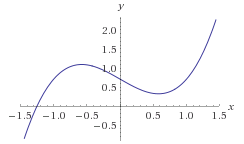
\includegraphics[width=0.48\textwidth]{newtonfail}
  \end{center}
  \caption{$f(x) = x^3 - x + \frac{\sqrt{2}}{2}$}
\end{wrapfigure}
We will select a ``bad'' initial guess such that if we start Newton's Method
from this guess, we will never converge to a solution.
Let our initial guess be $x_0 = 0$.
Note that this function has derivative $f'(x) = 3x^2 - 1$.
Thus plugging in our initial guess gives us
\begin{equation*}
  x_1 = x_0 - \frac{1}{f'(x_0)} f(x_0) = \frac{\sqrt{2}}{2}.
\end{equation*}
But then we encounter a problem once we use $x_1$ to determine $x_2$.
\begin{equation*}
  x_2 = x_1 - \frac{1}{f'(x_1)} f(x_1) = 0.
\end{equation*}
This brings us back to our initial guess!
So now Netwon's method will oscillate between $0$ and $\frac{\sqrt{2}}{2}$, and
it will not converge to a solution.

The additional conditions that we need for the convergence of Newton's Method
are given in a theorem by Kantorovitch.
In order to guarantee convergence, we need a bound on the second derivative of
the function $f$.
For completeness, let's state this theorem.

\begin{thm}[Kantorovitch]
  Let $E$ and $F$ be Banach spaces, $U$ be an open subset of $E$, and $f : U \to
  F$ be $C^1$.
  Suppose that $\bp{x}_0 \in U$ is a point where $[\Dif f(\bp{x}_0)] : E \to F$
  is an isomorphism.
  Set
  \begin{align*}
    h_0 &= -[\Dif f(\bp{x}_0)]^{-1}(f(\bp{x}_0)),\\
    \bp{x}_1 &= \bp{x}_0 + h_0,\\
    U_0 &= B_{\norm{h_0}}(\bp{x}_1).
  \end{align*}
  Then if the following hold:
  \begin{enumerate}
  \item $U_0 \subset U$
  \item $\norm{[\Dif f(\bp{y}_1)] - [\Dif f(\bp{y}_2]} \leq M$ for all
    $\bp{y}_1, \bp{y}_2 \in U_0$
  \item $\norm{f(\bp{x})} \norm{[\Dif f(\bp{x}_0)]^{-1}}^2 M \leq \frac{1}{2}$
  \end{enumerate}
  then the equation $f(\bp{x}) = 0$ has a unique solution in $U_0$, and Newton's
  method starting from $\bp{x}_0$ is defined for all $i$ and converges to this
  solution.
  If moreover we have
  \begin{equation*}
    \norm{f(\bp{x})} \norm{[\Dif f(\bp{x}_0)]^{-1}}^2 M = k < \frac{1}{2},
  \end{equation*}
  Then the method is \emph{superconvergent}.
  That is, if we put
  \begin{align*}
    C &= \frac{1 - k}{2(1 - 2k)}\norm{[\Dif f(\bp{x}_0)]^{-1}} M,\\
    \bp{x}_{i+1} &= \bp{x}_i + h_im\\
    h_{i+1} &= -[\Dif f(\bp{x}_i)]^{-1} f(\bp{x}_i),
  \end{align*}
  then $\norm{h_{i+1}} \leq C \norm{h_i}^2$.
\end{thm}
Note that superconvergence corresponds to doubling the number of correct digits
at each iteration.
Geometric convergence differs from superconvergence, as it adds only a fixed
number of significant figures at each iteration.
The interested reader can follow a proof given in \cite{hh09} and fill in some
minor details to apply it to this more general case.

In solving for the diffeomorphism $\Phi$ in the proof of Kolmogorov's theorem,
we will be using a similar technique to Newton's method.
Where with Newton's method we needed a bound on the second derivative, we will
need some type of analogous condition for our iterative process.
We need some way to measure ``size,'' that is, we need to choose a norm for our
functions.

First let's recall the definition of a Banach algebra.
\begin{defn}[Banach Algebra]
  Let $k$ be $\R$ or $\C$.
  A \emph{normed algebra} over $k$ is an algebra $\mathcal{A}$ over $k$ with a
  sub-multiplicative norm $\norm{\cdot}$.
  That is, for all $x, y \in \mathcal{A}$, we have
  \begin{equation*}
    \norm{xy} \leq \norm{x}\norm{y}.
  \end{equation*}
  If $\mathcal{A}$ is a Banach space, then it is called a Banach algebra.
\end{defn}
Let $X \subseteq \C^k$ be compact, and let the caligraphic letter $\mathcal{X}$
be the Banach algebra of continuous functions on $X$ that are analytic in the
interior and have the sup norm
\begin{equation*}
  \norm{f}_X = \sum_{\bp{x} \in X} |f(\bp{x})|.
\end{equation*}
Here we use the normal absolute value as the standard Euclidean norm on $\C^n$.


We consider three regions:
% TODO use these somewhere useful
\domains{}Denote by $\mathcal{B}_{\rho}$, $\mathcal{C}_{\rho}$, and
$\mathcal{A}_{\rho}$ the corresponding Banach algebras.
We can expand elements of $\mathcal{B}_{\rho}$ as power series, and elements of
$\mathcal{C}_{\rho}$ as Fourier series:
\begin{equation*}
  f(\bp{z}) = \sum_{\bp{k} \in \Z^n} f_{\bp{k}} \e^{2 \pi \i \bp{k} \cdot \bp{z}}.
\end{equation*}
This Fourier series expansion will be important in \cref{sec:dioph-diff-equat}.

Let's take a look at how we can bound derivatives of analytic functions,
analogous to how we use the second derivative to bound the derivative of
functions in Kantorovitch's Theorem.
We will use Cauchy's Inequalities on Balls.
\begin{thm}[Cauchy's Inequalities on Balls]
  If $f \in \mathcal{B}_{\rho}$, then
  \begin{align*}
    \norm{\Dif f}_{\rho - \delta} &\leq \frac{1}{\delta} \norm{f}_{\rho},\\
    \norm{\Dif^2 f}_{\rho - \delta} &\leq \frac{4}{\delta^2} \norm{f}_{\rho}.
  \end{align*}
  As a corollary, the case $\delta = \rho$ bounds the derivatives at the center
  of balls:
  \begin{align*}
    |\Dif f(0)| &\leq \frac{1}{\rho} \norm{f}_{\rho},\\
    |\Dif^2 f(0)| &\leq \frac{4}{\rho^4} \norm{f}_{\rho}.
  \end{align*}
\end{thm}
\begin{proof}
  % TODO expand on proof and include more details
  Take $\bp{z} \in B_{\rho - \delta}$ and $\bp{u} \in \C^n$.
  Since $B_{\delta}(\bp{z}) \subseteq B_{\rho}$, the function
  \begin{equation*}
    g : t \mapsto f(\bp{z} + t \delta \bp{u})
  \end{equation*}
  is defined on the unit disc.
  The normal Cauchy inequality implies that
  \begin{equation*}
    \delta|(\Dif f(\bp{z})) \bp{u}| = |g'(0)| \leq \norm{g}_{1} \leq
    \norm{f}_{\rho}.
  \end{equation*}
  Applying the argument twice gives the result for the second derivative:
  \begin{equation*}
    |\Dif^2 f(\bp{z})(\bp{u}, \bp{v})| \leq \frac{2}{\delta} \norm{\Dif f
      (\bp{z})(\bp{u})}_{\rho - \frac{\delta}{2}}|\bp{v}| \leq
    \frac{4}{\delta^2} \norm{f}_{\rho} |\bp{u}||\bp{v}|.
  \end{equation*}
\end{proof}

\section{Main Idea of the Proof}
\label{sec:main-idea-proof}

Let's take another look at the statement of Kolmogorov's theorem and recall
\cref{eq:sdiffeo}, where we have $H = h \circ \Phi$:
\begin{equation*}
  H(\bp{Q}, \bp{P}) = A + \omega \bp{P} + R(\bp{Q}, \bp{P}).
\end{equation*}
This equation is an equation for a diffeomorphism $\Phi$, and the proof involves
solving for this diffeomorphism.
We would like to use Newton's method to do this solving, but that in itself is
not quite sufficient for out purposes.
However, we can still do something with a similar flavor.

The proof uses an iterative process in which we obtain the diffeomorphism $\Phi$
as a limit of $\Phi_i$, where
\begin{equation*}
  \Phi_i = \phi_i \circ \phi_{i - 1} \circ \cdots \circ \phi_1.
\end{equation*}
Here, $\phi_i$ denotes the Hamiltonian flow $\phi_{g_i}$ for a Hamiltonian
function $g_i$.
This $g_i$ is the unknown for which we solve.

% TODO pause and take a moment to reflect on how we went from a diffeomorphism
% to a function.
Let's take a moment to pause and reflect on what was just done.
Instead of solving for a diffeomorphism $\Phi$, at each iteration we are solving
for a Hamiltonian function $g_i$.
This simplification is rather important, as a diffeomorphism can be a rather
complicated object.
The $g_i$ are much easier to reason about.
Furthermore, the map $\phi_{g_i}$ is itself a symplectic diffeomorphism.
% TODO continue reflection

At the $i$th iteration we have a Hamiltonian $\tilde{h} = \Phi_i^* h$.
We expand $\tilde{h}$ up to order $2$ in $\bp{p}$, and the coefficients are
Fourier series in $\bp{q}$.
We write $\tilde{h} = \tilde{h}_0 + \tilde{h}_1$, where
\begin{itemize}
\item $\tilde{h}_1$ has the terms constant or linear in $\bp{p}$, except the
  constant in $\bp{q}$,
\item $\tilde{h}_0$ is everything else.
\end{itemize}
We would very much like to eliminate $\tilde{h}_1$, but we won't be able to do
so by solving a linear equation.
Instead we will solve a linear equation for a function $g$ such that
$\phi_g^*\tilde{h}$ is ``better'' than $\tilde{h}$, in some reasonable sense of
``better.''

We expand $\phi_g^* \tilde{h}$ to first order in $g$.
This gives us
\begin{align*}
  \phi_g^* \tilde{h} &= \tilde{h} + \{g, \tilde{h}\} + o(|g|)\\
                     &= \tilde{h}_0 + \tilde{h}_1 + \{g, \tilde{h}_0\} + \{g,
                       \tilde{h}_1\} + o(|g|).
\end{align*}
We want to eliminate the terms, other than the term constant in $\bp{q}$, that
are not $O(|\bp{p}|)^2$.
Applying the standard Newton's method would necessitate solving the equation
\begin{equation*}
  \tilde{h}_1 + \{g, \tilde{h}_0\} + \{g, \tilde{h}_1\} \in o(|\bp{p}|).
\end{equation*}
But we will do something a bit different.

We can assume that anything we want is small as long as the choice is justified
by the resulting inequalities.
So suppose that $\{g, \tilde{h}_1\}$ is of order $2$ since $g$ and $\tilde{h}_1$
are both small.
Then the linear equation that we need to solve is
\begin{equation}
  \label{eq:dio-diff-first}
  \tilde{h}_1 + \{g, \tilde{h}_0\} \in o(|\bp{p}|).
\end{equation}
Thus we need to solve this \emph{Diophantine partial differential equation}.
Our ability to solve it relies on the Diophantine vectors that we saw previously
in \cref{sec:irrationality}.
Recall that we have the hypothesis $\omega \in \Omega_{\gamma}$ in the statement
of the theorem.
This hypothesis gives us the irrationality that is required for
\cref{eq:dio-diff-first} to have a solution.

\section{Diophantine Differential Equations}
\label{sec:dioph-diff-equat}

Let $g \in \mathcal{C}_{\rho}$.
We are going to be solving linear equations of the form
\begin{equation}
  \label{eq:dio-form}
  \Dif f(\omega) = \sum_{i = 1}^n \omega_i \pd{f}{q_i} = g,
\end{equation}
with $f \in \mathcal{C}_{\rho'}$ for some $\rho' < \rho$.
Recall, as was mentioned in \cref{sec:analytic-functions}, that since $f \in
\mathcal{C}_{\rho'}$ and $g \in \mathcal{C}_{\rho}$, we can write $f$ and $g$ as
Fourier Series.
\begin{align*}
  f(\bp{q}) &= \sum_{\bp{k} \in \Z^n} f_{\bp{k}} \e^{2 \pi \i \bp{k} \cdot
    \bp{q}},\\
  g(\bp{q}) &= \sum_{\bp{k} \in \Z^n} g_{\bp{k}} \e^{2 \pi \i \bp{k} \cdot \bp{q}}.
\end{align*}
The solution is given by
\begin{equation}
  \label{eq:dio-sol}
  f_{\bp{k}} = \frac{1}{2 \pi \i (\bp{k} \cdot \omega)}g_{\bp{k}}.
\end{equation}
We need $g_0$ to be zero.
Then $f_0$ is arbitrary, and otherwise the series for $f$ is unique.

Take note of the $(\bp{k} \cdot \omega)$ in the denominator of \cref{eq:dio-sol}
and compare this expression to our definition of a Diophantine vector in to
\cref{eq:diovec}.
Dividing by zero in \cref{eq:dio-sol} would mean that there is no solution.
So we need the Diophantine condition for the vector $\omega$ to ensure that we
do not divide by zero in \cref{eq:dio-sol}.
Hence the convergence properties of $f$ depend on the Diophantine properties of
$\omega$.
Without this condition, we would be unable to find solutions to these equations.

But even though this condition gives us convergence for $\rho$, we might not
have boundedness.
So we need some $\rho' < \rho$ where we have boundedess.
But we must choose $\rho'$ large enough so that the limit is nonempty.
Thus we have a trade off.
We must be able to pick $\rho'$ correctly in order for our iterative method of
solving the equation converges to a solution.
Thus the choice of $\rho'$ must be done rather ``carefully.''
We will avoid writing out all of the details and instead direct the reader to
\cite{hi02}.
But we will develop the proposition that we need for choosing this $\rho'$, and
in \cref{sec:solving-equations} we will see how to use it.

The following tool, which we then prove, is what we use for making our careful
choice of $\rho'$.
\begin{prop}
  \label{prop:tool}
  If $g \in \mathcal{C}_{\rho}$ and $\epsilon \in \Omega_{\gamma}$, then for all
  $\delta$ such that $0 < \delta < \rho$, we have the following two
  inequalities:
  \begin{align*}
    \norm{f}_{\rho - \delta} &\leq \frac{\kappa_n}{\gamma
                               \delta^{2n}}\norm{g}_{\rho},\\
    \norm{\Dif f}_{\rho - \delta} &\leq \frac{\kappa_n}{\gamma \delta^{2n + 1}}
                    \norm{g}_{\rho}.
  \end{align*}
  Here, $\kappa_n$ is a constant that depends only on $n$.
\end{prop}
\begin{proof}
  For $\bp{y} \in \R^n$ with $|\bp{y} \leq \rho$ (in particular $\bp{y} = \rho
  \frac{\bp{k}}{|\bp{k}|})$, the function
  \begin{equation*}
    \bp{q} \mapsto g(\bp{q} - \i \bp{y})
  \end{equation*}
  is continuous and periodic in $\bp{q}$ of period $1$.
  This function can be written
  \begin{equation*}
    g(\bp{q} - \i \bp{y}) = \sum_{\bp{k} \in \Z^n} g_{\bp{k}} \e^{2 \pi \i
      \bp{k} \cdot (\bp{q} - \i \bp{y})} = \sum_{\bp{k} \in \Z^n}
    \left(g_{\bp{k}} \e^{2 \pi \bp{k} \cdot \bp{y}} \right) \e^{2 \pi \i \bp{k}
      \cdot \bp{q}}.
  \end{equation*}
  By Parseval's theorem, we have
  \begin{equation*}
    \norm{g}_{\rho}^2 \geq \int_{\T^n} |g(\bp{q} - \i \bp{y})|^2 |\dif ^n
    \bp{q}| = \sum_{\bp{k} \in \Z^n} |g_{\bp{k}}|^2 \e^{4 \pi \bp{k} \cdot \bp{y}}.
  \end{equation*}
  Since the series has positive numbers, we have
  \begin{equation*}
    \norm{g}_{\rho}^2 \geq |g_{\bp{k}}|^2 \e^{4 \pi \rho|\bp{k}|}.
  \end{equation*}

  Using the Diophantine-ness of $\omega$ and the Fourier coefficients
  $f_{\bp{k}}$, we have
  \begin{equation*}
    |f_{\bp{k}}| \leq \frac{1}{2 \pi \gamma} \norm{g}_{\rho} |\bp{k}|^n \e^{-2
      \pi |\bp{k}| \rho}.
  \end{equation*}

  Next we split the proposition into two parts: the first part dealing with the
  $f$ case and the second part dealing with the $\Dif f$ case.

  First we handle the case for $f$.
  For $|\bp{q}| \leq \rho - \delta$, we can write
  \begin{align*}
    \left| f_{\bp{k}} \e^{2 \pi \i (\bp{k} \cdot \bp{q})} \right|
    &\leq \sum_{\bp{k} \in \Z^n} \frac{|\bp{k}|^n}{2\pi\gamma} \norm{g}_{\rho}
      \e^{-2 \pi \rho |\bp{k}|(\rho - \delta)}\\
    &= \frac{\norm{g}_{\rho}}{2 \pi \gamma} \sum_{\bp{k} \in \Z^n} |\bp{k}|^n
      \e^{-2 \pi |\bp{k}|\delta}.
  \end{align*}
  We then rewrite the sum on the right:
  \begin{equation*}
    \sum_{\bp{k} \in \Z^n} |\bp{k}|^n \e^{-2 \pi |\bp{k}|\delta} = \frac{1}{(2
      \pi \delta)^{2n}} \left((2 \pi \delta)^n \sum_{\bp{k}' \in 2 \pi \delta
        \Z^n} |\bp{k}'|^n \e^{-|\bp{k}'|} \right).
  \end{equation*}
  As $\delta \to 0$, the expression inside the parentheses approaches
  \begin{equation*}
    \int_{\R^n} |\bp{x}|^n \e^{-|\bp{x}|} |\dif^n \bp{x}|.
  \end{equation*}
  Since the integral is convergent there exist $\kappa_n'$ such that for $\delta
  \leq 1$, it holds that
  \begin{equation*}
    \sum_{\bp{k} \in \Z^n} |\bp{k}|^n \e^{-2 \i |\bp{k}|\delta} \leq
    \frac{\kappa_n'}{(2 \pi \delta)^{2n}}.
  \end{equation*}
  We now have
  \begin{equation*}
    \norm{f}_{\rho - \delta} \leq \frac{\kappa_n}{(2 \pi \delta)^{2n}}
    \frac{\norm{g}_{\rho}}{2 \pi \gamma}.
  \end{equation*}
  Thus we are finished with the $f$ part of the proof.

  The $\Dif f$ part of the proof is similar.
  We use
  \begin{equation*}
    \Dif f(\bp{q})(\bp{u}) = 2 \pi \i \sum(\bp{k} \cdot \bp{u}) f_{\bp{k}} \e^{2
      \pi \i (\bp{k} \cdot \bp{q})}.
  \end{equation*}
  Then we obtain the inequality
  \begin{equation*}
    |\Dif(\bp{q})(\bp{u})| \leq \frac{|\bp{u}| \norm{g}_{\rho}
      \kappa_n''}{\gamma(2 \pi \gamma)^{n+1}}.
  \end{equation*}
  Analogous to the first part of the proof, the integral
  \begin{equation*}
    \int_{\R^n} |\bp{x}|^{n+1} \e^{-|\bp{x}| |\dif^n\bp{x}|}
  \end{equation*}
  is convergent.
  Thus $\kappa_n''$ exists.

  To complete the proof of the proposition, take
  \begin{equation*}
    \kappa_n := \max \left\{\frac{\kappa_n'}{(2n)^{2n}},
      \frac{\kappa_n''}{(2n)^{2n+1}}\right\}.
  \end{equation*}
\end{proof}

\section{Solving Equations}
\label{sec:solving-equations}

Let's return to our previous equation
\begin{equation*}
  h_1 + \{g, h_0\} \in O(|\bp{p}|^2).
\end{equation*}
This equation is the Diophantine differential equation that we had before in
\cref{eq:dio-diff-first}, but without tildes and with $o(|\bp{p}|)$ replaced by
$O(|\bp{p}|^2)$, which is equivalent since our functions are analytic.
The unknown is $g$, which we take to be degree $1$ in $\bp{p}$:
\begin{equation*}
  g = \lambda \bp{q} + X(\bp{q}) + \sum_{i=1}^n Y_i(\bp{q}) p_i.
\end{equation*}
Note that only the linear terms of $g$ contribute to the linear terms of $\{g,
h_0\}$.
The unknowns are $\lambda$, $X$, and $Y_i$.
We can expand $X$ and $Y_i$ as Fourier series, since they are functions of
$\bp{q}$ only.

Let $a \in \R$, $\omega \in \Omega_{\gamma}$, $R(\bp{q}, \bp{p}) \in
O(|\bp{p}|^3)$, and $\overline{A} = 0$, where $\overline{A}$ is the average of
$A$ on the torus $\bp{p} = 0$.
We can then write
\begin{align*}
  h_0(\bp{q}, \bp{p}) &= a + \omega \bp{p} + \frac{1}{2} \bp{p} \cdot C(\bp{q})
                        \bp{p} + R(\bp{q}, \bp{p}),\\
  h_1(\bp{q}, \bp{p}) &= A(\bp{q}) + B(\bp{q}) \bp{p}.
\end{align*}
We then have
\begin{equation*}
  (h_1 + \{g, h_0\}) (\bp{q}, \bp{p}) = \omega \cdot \lambda + A(\bp{q}) + \Dif
  X(\bp{q}) (\omega) + \Big( B(\bp{q}) + \big(\lambda + \Dif X(\bp{q}) \big)
  C(\bp{q}) + \omega \Dif Y(\bp{q}) \Big) \cdot \bp{p} + O(|\bp{p}|^2).
\end{equation*}

We need to solve the equations
\begin{align}
  \label{eq:fst-to-solve}
  \Dif X(\bp{q}) (\omega) &= - A(\bp{q})\\
  \label{eq:snd-to-solve}
  \Dif Y(\bp{q}) (\omega) &= -B(\bp{q}) - \big(\lambda + \Dif
     X(\bp{q})\big)C(\bp{q})
\end{align}
for $X$ and $Y_i$, $i = 1, \ldots, n$.
These are Diophantine differential equations.
To see this, let's write these in the form of \cref{eq:dio-form}, which we have
already discussed how to solve.

For \cref{eq:fst-to-solve}, we can write
\begin{equation*}
  \sum_i \omega_i \pd{X}{q_i} = -A(\bp{q}).
\end{equation*}
Second, we note that \cref{eq:snd-to-solve}, consists of $n$ differential
equations.
These equations can be written in the form
\begin{equation*}  
  \sum_i \omega_i \pd{Y_i}{q_i} = -B_j(\bp{q}) - \sum_i C_{i,j}(\bp{q}) \left(
  \lambda_i + \pd{X}{q_i} \right).
\end{equation*}
We will solve the first equation, \cref{eq:fst-to-solve}, and then plug in this
solution to help solve \cref{eq:snd-to-solve}.

Since we have the hypothesis $\overline{A} = 0$, we can solve the first
equation.
We can find a unique $X$ such that $\overline{X} = 0$ and that for all $\delta$
with $0 < \delta < \rho$, the bounds
\begin{align*}
  \norm{X}_{\rho - \delta} &\leq \frac{\kappa_n \epsilon}{\gamma \delta^{2n}},\\
  \norm{\Dif X}_{\rho - \delta} &\leq \frac{\kappa_n \epsilon}{\gamma
                   \delta^{2n+1}},
\end{align*}
are satisfied.

Now we want to solve \cref{eq:snd-to-solve}.
In order to solve it, we need its right hand side to be zero.
For this we need to choose $\lambda$.
Set
\begin{equation*}
  \lambda = - \overline{C}^{\,-1} \overline{(B + (DX)C)}.
\end{equation*}
Then we have
\begin{equation*}
  \norm{B - (DX)C}_{\rho - \delta} \leq \epsilon + \frac{\kappa_n \epsilon}{m
    \gamma \delta^{2n+1}} \leq \frac{2 \kappa_n \epsilon}{m \gamma \delta^{2n +
  1}}.
\end{equation*}
This inequality gives us
\begin{equation*}
  |\lambda| \leq \frac{2\kappa_n \epsilon}{m^2 \gamma \rho^{2n+1}} \leq \frac{2
    \kappa_n \epsilon}{m \gamma \delta^{2n + 2}}.
\end{equation*}
From here we get
\begin{align*}
  \norm{B - (\lambda + DX)C}_{\rho - \delta}
  &\leq \norm{B - (DX)C}_{\rho - \delta} + \norm{\lambda C}_{\rho - \delta}\\
  &\leq \frac{2 \kappa_n \epsilon}{m \gamma \delta^{2n + 1}} + \frac{2\kappa_n
    \epsilon}{m^3 \gamma \delta^{2n+1}}\\
  &\leq \frac{4 \kappa_n \epsilon}{m^3 \gamma \delta^{2n+1}}.
\end{align*}
Now we use the tool that we developed in the form of \cref{prop:tool}.
This proposition allows us to fund $Y \in \mathcal{C}_{\rho - 2\delta}^n$ such
that $\overline{Y} = 0$ and that the following estimates are satisfied:
\begin{align*}
  \norm{Y}_{\rho - 2\delta} &\leq \frac{4\kappa_n^2 \epsilon}{m^3 \gamma^2
                              \delta^{4n+1}}\\
  \norm{\Dif Y}_{\rho - 2\delta} &\leq \frac{4\kappa_n^2 \epsilon}{m^3 \gamma^2
                    \delta^{4n+2}}.
\end{align*}

Let's summarize what we have done to solve these equations.
These equations are Diophantine differential equations.
The hypothesis $\overline{A} = 0$ allows us to solve \cref{eq:fst-to-solve} and
to find $X \in \mathcal{C}_{\rho'}$ for all $\rho' < \rho$.
We then substitute into the second equation.
We can then determine $\lambda$ so that the averages of the right-hand sides in
the $n$ are all zero.
Then we can solve the second equation and find $Y_i \in \mathcal{C}_{\rho''}$
for all $\rho'' < \rho'$.
Iterating the process requires choosing $\rho'$ and $\rho''$ ``carefully.''
The remaining details are left to \cite{hi02}.

\section{Conclusion}
\label{sec:conclusion}

The proof by Hubbard and Ilyshenko in \cite{hi02} is considerably shorter than
many previous proofs, and solely by following it without considering the work
before it we may miss out on what make it so useful, and why the ideas it
contains are so powerful.
% TODO cite Arnold's original proof and many other proofs of the theorem
We can tell that the proof is difficult merely by the fact that Moser's proof,
given in %TODO cite
involves functions that are $333$ times differentiable.

With everything that we have discussed, the statement of Kolmogorov's Theorem
should now be very much readable, and the main ideas of the proof should be
understandable.
We have an equation that we solve for a diffeomorphism.
This equation is solved iteratively using an analogue of Newton's Method.
We used analytic functions in order for this technique to converge properly,
analogous to how we would need to bound the second derivative if we were to
apply Kantorovitch's Theorem when using Newton's Method.
And we need the Diophantine vectors in order to avoid dividing by zero when
solving for our Fourier coefficients.

% TODO concluding paragraph

% TODO add works to bibliography and update references throughout paper
\nocite{*}
\bibliographystyle{plain}
\bibliography{bibliography}

\end{document}

%%% Local Variables:
%%% mode: latex
%%% TeX-master: t
%%% End:
